\documentclass{standalone}
\usepackage{tikz}
\usepackage{ctex,siunitx}
\setCJKmainfont{Noto Serif CJK SC}
\usepackage{tkz-euclide}
\usepackage{amsmath}
\usetikzlibrary{patterns, calc}
\usetikzlibrary {decorations.pathmorphing, decorations.pathreplacing, decorations.shapes,}
\begin{document}
\small
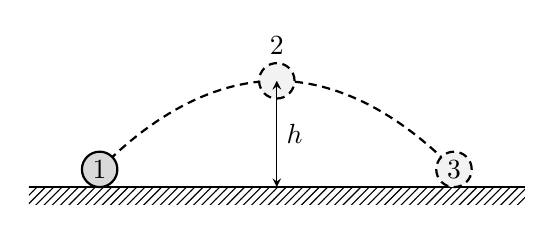
\begin{tikzpicture}[>=stealth,thick,scale=0.9]
  \fill [pattern = north east lines] (-1,-.25) rectangle (6,0);
  \draw (-1,0)--(6,0);
  \draw [densely dashed] (0,0.25) parabola [bend pos=0.5] bend (2.5,1.5) (5,0.25);
  \draw [fill=gray!30] (0,.25) node {1} circle (.25) ;
  \draw [densely dashed, fill=gray!10] (5,.25) circle (.25) node  {3};
  \draw [densely dashed,fill=gray!10] (2.5,1.5) circle (.25) node  [above=2mm] {2};
  \draw [thin,<->] (2.5,1.5)--node [right]{$h$}(2.5,0);
\end{tikzpicture}
\end{document}